\chapter{Overview of the hardware}

\section{Features of the DE10-Nano development board}

On the board, numerous devices are made available to the user. Some of them will be very 
interesting for this work: the Cyclone V FPGA that includes a programmable part (the programmable 
logic) and an ARM processor (A in Figure \ref{fig:de10/de10_features}) that is
basically the main component of the system as almost everything on the board is driven by it. It is
also where all the hardware designed in the work resides. The 1GB DDR3 RAM (B) which is used 
by the ARM side of the FPGA. An ethernet port (C) which can be
useful to connect to the ARM processor from any external environment. For instance, SSH can be used
to connect to it if the installed system can handle it. Then there are the SD card reader and the SD 
card (D, on the other side of the PCB). The SD card consists in the mass storage of this board. The
one used offers 8GB of memory. Another important component is the HDMI output (E) that can be used
from the programmable logic side of the Cyclone V. Other less important devices, mainly IOs are 
avaible: General Purpose Input / Output pins (GPIOs), LEDs, buttons and switches. All of these 
devices are discussed at some point in this report. The ones that are not listed (such as the Inertial
Measurement Unit, IMU) haven't been used.

\begin{figure}[H]
    \centering
    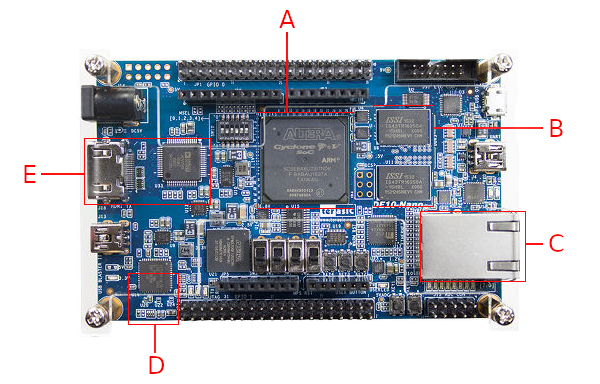
\includegraphics[scale=0.5]{Chapter1-Hardware/res/de10_nano.png}
    \caption{DE10 Nano development board main features}
    \label{fig:de10/de10_features}
\end{figure}

\section{Programmable logic devices}

Field Programmable Gate Arrays (FPGAs) are a type of Programmable Logic Device (PLD) which are, as 
the name suggests, programmable logic circuits. Programmable means that the user can choose which 
circuitry will be implemented in these devices and as it will be shown in this chapter, some of 
these devices are very versatile! They can implement almost any kind of digital circuit.

PLDs come in different forms but follow a similar pattern for most types. In fact, they almost all 
are composed of an AND array and an OR array that are both programmable or not. Here, a discussion 
of these different types and their evolution will be made to arrive at FPGAs and show the advantages 
and disadvantages compared to other technologies.

\subsection{ROM based PLDs}

This first type is very simple, as shown in Figure \ref{fig:fpga/pld_rom_external}. In fact, the 
circuit, which can only be combinatorial, will be simulated by a ROM. Each address corresponds to 
an input of the circuit and each word in memory to an output of the circuit. The ROM therefore 
simply contains the truth table of the logic circuit to be implemented.

\begin{figure}[H]
    \centering
    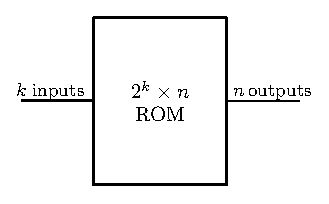
\includegraphics[scale=1.2]{Chapter1-Hardware/res/pld_rom_external}
    \caption{An external view of ROM based PLDs}
    \label{fig:fpga/pld_rom_external}
\end{figure}

The inside of a $2^2 \times 4$ ROM can be seen as a 2-to-4 decoder followed with a 4-by-4 OR gates 
array, as shown in Figure \ref{fig:fpga/pld_rom_internal}, where the connections in the array are configurable. They can be opened or closed during the
programmation of the device. The decoder can be interpreted as the AND gates array here. Thus, the
AND gates array is fixed and the OR gates array is programmable for this kind of devices.

In the example of Figure \ref{fig:fpga/pld_rom_internal}, the array is represented by a grid. All horizontal lines represent a 1-bit signal
that can be connected to an OR gate. The signal is connected if a red x is present at the connection
point. As can be seen, the OR gates array is here programmed to describe the truth tables of these 
boolean equations

\begin{equation*}
    \begin{cases}
        A_0& = I_0 \cdot \bar{I_1} \\
        A_1& = \bar{I_1} \\
        A_2& = 0 \\
        A_3& = \bar{I_0} \cdot I_1
    \end{cases}
\end{equation*}

Obviously, real devices contain a lot more signals and gates to be cost effective and useful. 
As stated previously, the ROM PLDs can only represent combinatorial circuits. There is no register
or feedback loop in the circuits that are described with this technology.

\begin{figure}[H]
    \centering
    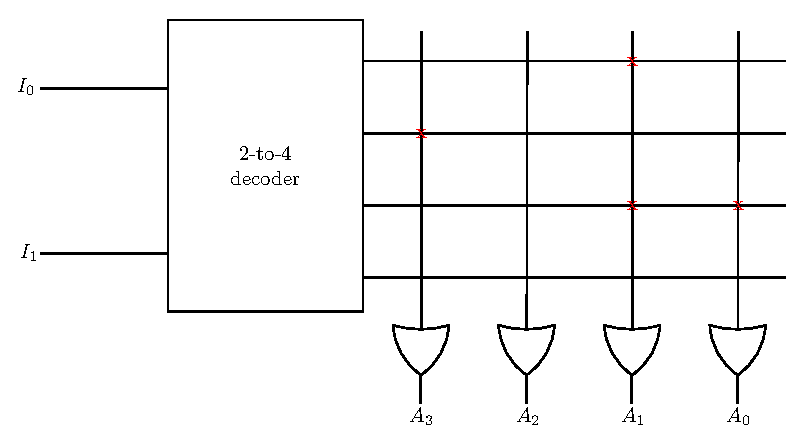
\includegraphics[scale=0.8]{Chapter1-Hardware/res/pld_rom_internal}
    \caption{An internal view of ROM based PLDs}
    \label{fig:fpga/pld_rom_internal}
\end{figure}

\subsection{PAL and PLA}

The Programmable Array Logic (PAL) and Programmable Logic Array (PLA) devices differ from the ROM 
based PLDs as they both have a programmable AND gates array. However, only the PLAs have both AND and
OR gates arrays that are programmable, the OR array is not programmable for PALs. The PLAs are thus 
the most flexible devices of the three.
As expected, this flexibility makes them also more complex and complicated to program. The outputs
of these devices can often be complemented through programmation too. It should also be notticed
that both the inputs and the inverted inputs are directly available in the arrays here, as visible
in Figure \ref{fig:fpga/pld_pla_internal}. These small additions greatly increase the possibilities
of such devices as programmable logic wont be used for that purpose.

\begin{figure}[H]
    \centering
    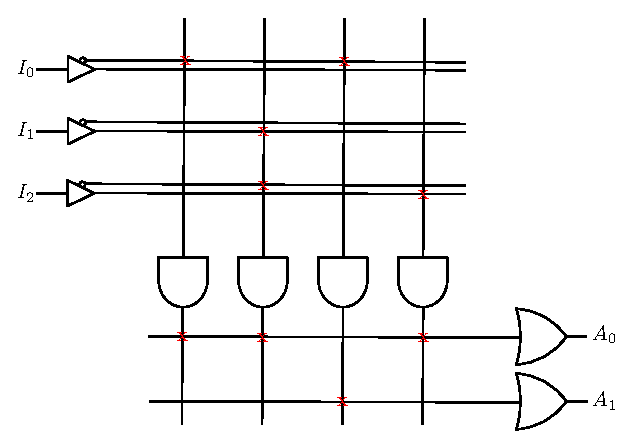
\includegraphics[scale=0.8]{Chapter1-Hardware/res/pld_pla}
    \caption{An internal view of PLAs}
    \label{fig:fpga/pld_pla_internal}
\end{figure}

\subsection{Programming methods}

It is very interesting to have programmable devices but it is even better when one can program them 
so this section contains a brief discussion of the common different programming techniques.
 
Initially, these devices were mainly programmable in two ways. The first was to use fuses and 
anti-fuses at each interconnection. The user then had to apply destructive currents to the right 
places for the fuses to open the connections and the anti-fuses to close them. The second method was 
to leave it to the user to complete the IC design. One would then make a mask to select which 
interconnects to open and close during a litography process. To provide some examples, the fuse 
methods are used in PROMs and 
masks for ROM based PLDs. Both of these programming methods make the devices non-erasable, which at 
the same time makes them non-reprogrammable. However, they are both non-volatile which can be an 
advantage when the user don't want any boot latency at startup, as no programmation is done at boot
time.

Later, other programming techniques were developed following the emergence of transistors. Indeed, 
these transistors are placed at the interconnections and controlled by their gate with the help of 
a bit kept in a memory. The memory can then be programmed to define the behaviour of the connections 
without them being frozen forever. As the memory is usually SRAM, the devices become reprogrammable
but still volatile. Other technologies have subsequently made it possible to have non-volatile 
memory in addition to memory by using, for example, floating gate transistors. These two types of 
interconnections are usually configured by applying a high current to set or reset the memory state. 

\section{The case of FPGAs}

Now that an introduction to PLDs and programming methods has been made, it is time to get to the 
heart of the matter with a description of FPGAs. In this section, it will be tried to be general 
enough to cover the operation of a large number of FPGAs. More details will be given in the next 
section that will be about the FPGA used for the realization of this master thesis.

FPGAs are fascinating yet complex devices. Indeed, they have three main programmable levels. These 
three levels will be discussed in turn, starting with the programmable logic blocks, then the 
programmable interconnect and finally the programmable I/Os. 

\subsection{Programmable logic blocks}

Programmable blocks are present in very large numbers in modern FPGAs (commonly tens to hundreds of 
thousands). They are the basic elements of the circuits implemented on FPGAs. Due to their 
architecture, which can be seen in Figure \ref{fig:fpga/fpga_block}, they allow both combinational 
and sequential circuits to be implemented. 

\begin{figure}[H]
    \centering
    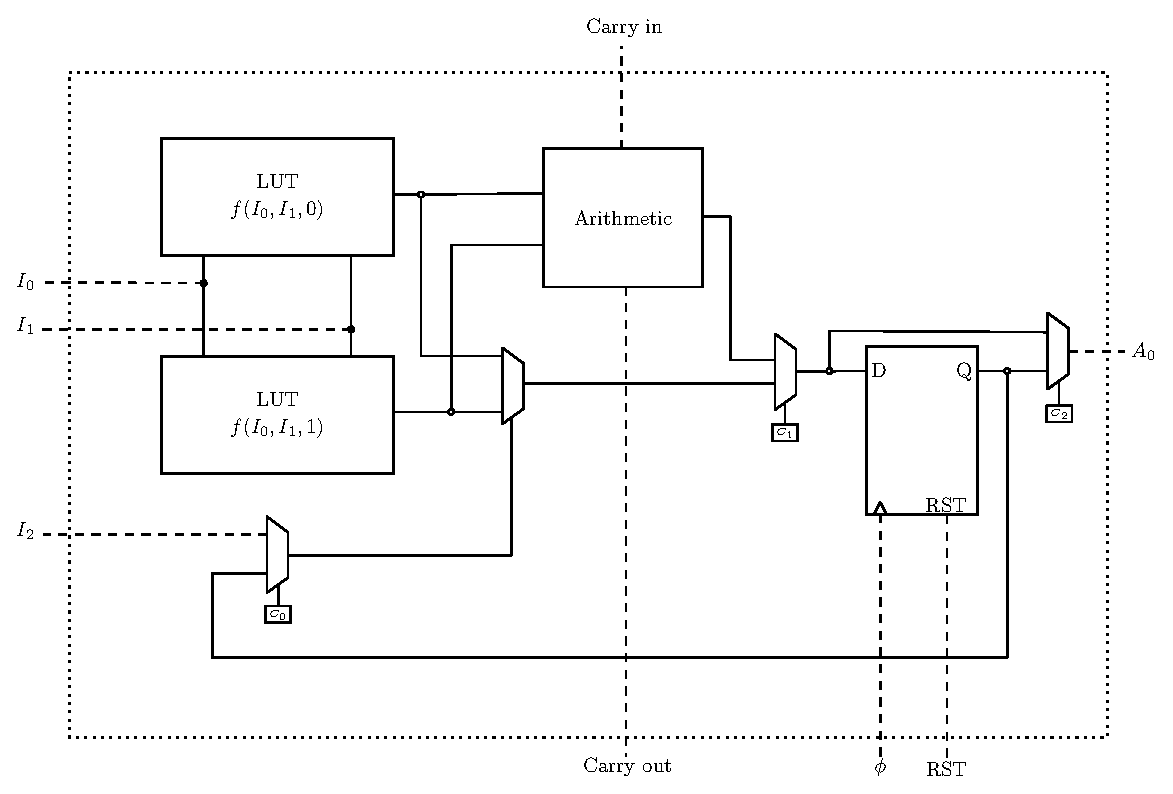
\includegraphics[scale=0.8]{Chapter1-Hardware/res/fpga_block}
    \caption{An FPGA programmable logic block}
    \label{fig:fpga/fpga_block}
\end{figure}

The combinatorial part of the circuits is implemented using a LookUp Table (LUT). The truth table is 
simply stored in this LUT as for the ROM PLDs but the bits are now stored in SRAM. If one LUT is 
not sufficient, the logic function can be implemented on several LUTs connected at the output by a 
multiplexer that is controlled by the remaining inputs. This is made fully valid by Shannon's 
expansion theorem. 

\begin{theorem}
    Any boolean function $f(x_1, x_2, ..., x_n)$ can be expressed as 
    \begin{equation*}
        f(x_1, x_2, ..., x_n) = x_n \cdot f(x_1, x_2, ..., x_{n - 1}, 1) + \bar{x_n} \cdot 
        f(x_1, x_2, ..., x_{n - 1}, 0)
    \end{equation*}
\end{theorem}

As shown in Figure \ref{fig:fpga/fpga_block}, the blocks also have an arithmetic sub-block and a 
register. Having this arithmetic block in each single programmable block greatly increases the 
efficiency of the FPGAs and reduces the latency of the blocks, even if most of the time these circuits are 
simple carry adders. Fixed hardware is always faster than programmable one as they are better 
optimized. In addition to the programmable LUTs, other configuration bits are available to control
the behaviour of the multiplexers: $C_1$, $C_2$ and $C_3$ allowing respectively to add a feedback 
loop to the block, to select the result of the boolean function or that of the arithmetic sub-block 
and to make the output of the block registered or not.

In brief, these blocks are the heart of the FPGA. All their features and configuration bits allow 
them to describe almost any kind of digital circuit in an efficient way.

\subsection{Non-programmable blocks}

Other non-programmable or less programmable blocks are also available on the FPGA. They are divided 
into two main groups: memories and utilities. Memories are simply blocks that can store data. A 
specific discussion of these memory blocks will be made in a later section. On the utility side, 
there can be a wide variety of blocks: multipliers, PLLs, DSPs and even whole CPUs. In short, 
enough to make FPGAs even more powerful!

\subsection{Programmable interconnect}

Programmable blocks are very versatile and efficient, but they need to be connected to each other to 
make large circuits. As can be seen in Figure \ref{fig:fpga/fpga_interconnect}, the blocks are 
positioned on a grid and the interconnection passes around them. 

\begin{figure}[H]
    \centering
    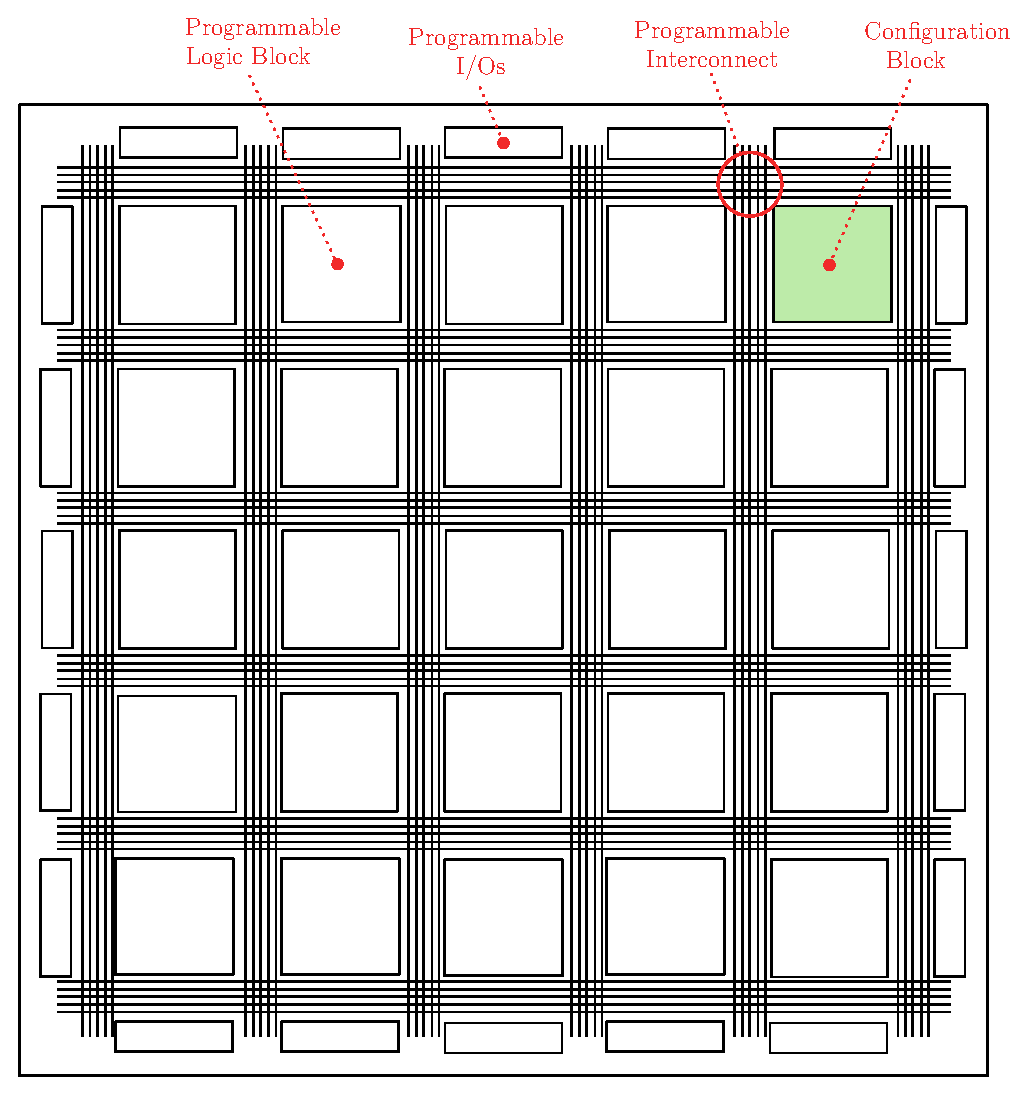
\includegraphics[scale=0.6]{Chapter1-Hardware/res/fpga_interconnect}
    \caption{High level view of an FPGA}
    \label{fig:fpga/fpga_interconnect}
\end{figure}

For this purpose, there is the programmable interconnection that will allow the signals to be routed 
from one block to another. To do this, configurable switches are placed at the crossings of the 
tracks. However, everything must be connected, whether the blocks are close or distant. As this 
cannot be done directly without causing problems in terms of time and power constraints, several 
hierarchical connection levels are present. However, in order to keep the explanations simple, it 
will be considered here that there is only one level. It should also be noted that each switch adds 
latency to the signal, so the interconnection is optimised to limit the number of switches between 
blocks. 

In addition to this configurable interconnection, there are also tracks to bring global signals 
everywhere. Among these signals are the clock, the resets, ... On a more local level, some signals 
are also shared between the blocks. These include, for example, the carry signals of the arithmetic 
sub-blocks.

\subsection{Programmable I/Os}

Now that almost the entire interior of the FPGA has been described, all that remains is to connect 
it to the outside. This is why there are these I/O pins all around the FPGA in Figure 
\ref{fig:fpga/fpga_interconnect}. These as well as the other parts of the FPGA are also 
configurable. As it is desirable for the FPGA to adapt to a wide variety of external hardware, these 
pins can be configured to the standard used. They can also be used as input, output, bi-directional, 
differential pairs, ... In short, they allow a large number of configurations so that the designed 
circuit can be adapted and coupled with a maximum of other circuits.

\subsection{Programmation of the FPGA}

Due to their complexity, the configuration circuitry of the FPGA is just as complex. For this 
reason, few details will be provided in this section. That said, it should be noted that part of 
the FPGA is assigned to this function. This block takes care of configuring all the 
configuration bits in the relevant memories. However, since the memories holding the configuration 
within the FPGA are volatile, it will often be necessary to couple a non-volatile memory to the 
FPGA to retain its configuration. The configuration will therefore have to be re-configured each 
time the FPGA is rebooted, which can create some latency. It is also important to note that the 
memory holding the configuration must be relatively large, as the number of configuration bits is 
very large. More details on compiling designs and configuring FPGAs in practice will be given in a 
later section.

This closes the theoretical discussion on FPGAs. As repeated several times, FPGAs are extremely 
powerful and configurable. This allows them to describe a large number of circuits and to adapt to
many existing circuits. Another advantage is that they are massively parallel due to their 
structure. Despite all these 
advantages, FPGAs still have some drawbacks. One of them is cost. Some FPGAs can cost several 
thousand euros. The complexity and difficulty of access is another problem for designers, the 
datasheets are numerous and extremely long, the tools are also numerous and not always easy to use. 
Electrical power requirements and start-up latency are also two other factors that must be taken 
into account when a user chooses an FPGA for circuit development. Nothing is perfect, not even 
FPGAs.

\section{Inside Cyclone V}

\subsection{Programmable logic side}

In the Cyclone V, things are a little more complicated than previously explained but are still quite 
accessible. In fact, the programmable logic blocks will be replaced here by Logic Array Blocks (LAB) 
which will themselves be made up of ten Adaptive Logic Modules (ALMs) which are the equivalent of 
the programmable logic blocks studied previously. A high level view of the LAB units is given in
Figure \ref{fig:cyc5/lab}. In the LAB, the different ALMs, the inputs and outputs of the LAB, can be 
interconnected at the user's convenience.

\begin{figure}[H]
    \centering
    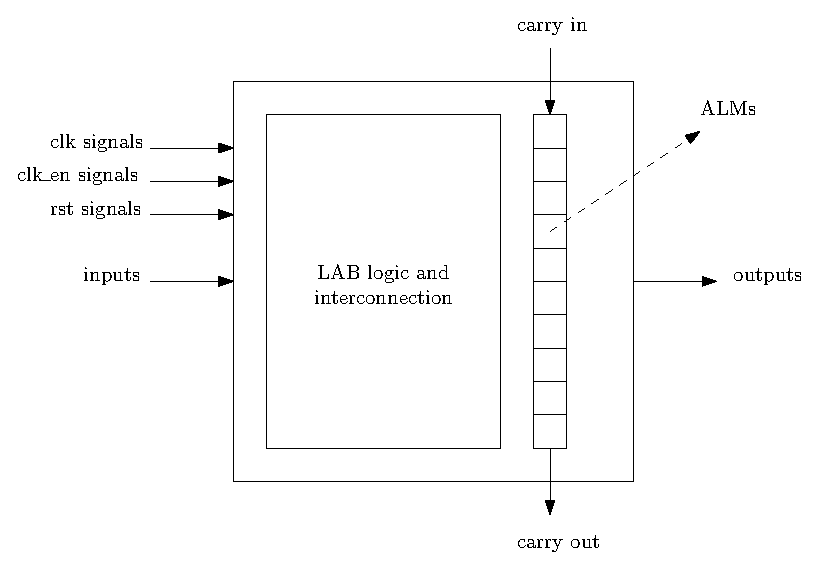
\includegraphics[scale=0.8]{Chapter1-Hardware/res/lab_block.eps}
    \caption{High level view of a LAB unit}
    \label{fig:cyc5/lab}
\end{figure}

There is also another type of LAB, the Memory LAB (MLAB) which allows to describe SRAM. They can 
store up to 640 bits and represent 25\% of all the LABs present on the Cyclone V. These MLABs do not 
have memory instead of the ten ALMs, they also have the ten ALMs and all the logic necessary 
to use them. They are a superset of LAB somehow.

These LABs (and MLABs) are placed in the FPGA fabric in an array as explained in the previous 
section. However, it should be noted that the array is not symmetrical with respect 
to the vertical and horizontal connections at the local level (this part was not detailed 
previously). Indeed, the horizontal connections aim to connect the blocks close to each other by 
ensuring a high speed of operation. These are the inputs and outputs that are mainly linked to it. 
The columns, although they are also fast, are mainly used for carry signals. At the local level, a 
LAB can have control over 30 ALMs: its own ten, and the ten of its two horizontal neighbors. This
allows to build very complex logic in a restricted space. Of course, a more global interconnection 
allows all LABs to be connected together. There are many more details about the internal 
connections of the LABs that could be discussed, but these are not explained in this report.

Concerning the ALMs, as just said, they are very similar to the Logic Array Blocks of 
the previous section. The main differences are that they accept more inputs, up to eight. The 
internal arithmetic block is in fact two separate adders and four registers are provided in each ALM. 
Depending on their configuration (done during the programming process), ALMs will be adapted to 
specialize in a functionality to make the circuits more efficient (for example more entries, an 
optimization for arithmetic, shared arithmetic with an input of the adder that is fed by an input 
of the ALM, ...). 

\subsubsection*{Other blocks}

The LAB blocks are very customizable and extremely numerous on the Cyclone 5. However, there are 
several other types of blocks that are worth listing and briefly explaining. The overall structure 
of the Cyclone V FPGA is shown in Figure \ref{fig:cyc5/structure}.

\begin{figure}[H]
    \centering
    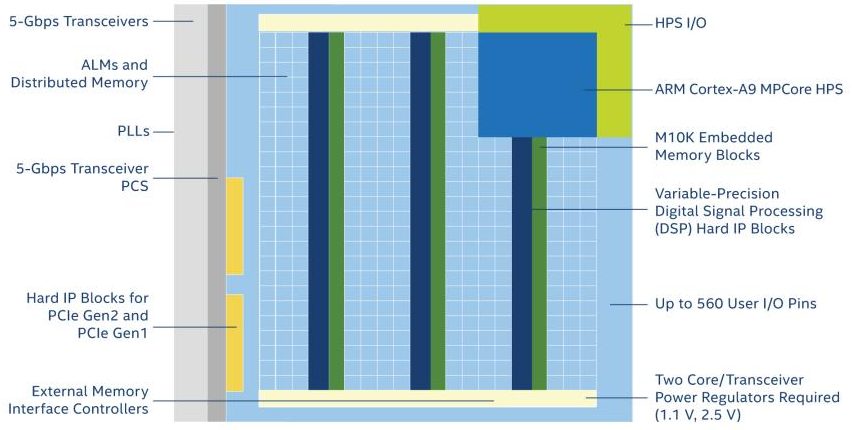
\includegraphics[scale=0.6]{Chapter1-Hardware/res/cycv_structure.PNG}
    \caption{Overall structure 
    of the Cyclone V FPGA}
    \label{fig:cyc5/structure}
\end{figure}

The largest block visible on the diagram is the one at the top right which represents the entire ARM
system, this block will be discussed in the section just after this one. Then one can see many dark 
green columns that designate the M10K memories. These memories are the main source of on-chip 
storage, a sub-section of this chapter being dedicated to the memories, they will be studied in more 
detail there. The PLLs are also visible in the light gray band on the left. PLLs allow to 
generate clocks at a given frequency from a reference clock. Again, this unit will be studied later. 
Another element present in large quantities is represented by the dark blue columns. It is the 
Digital Signal Processing (DSP) Hard IP Blocks. These blocks have a multitude of functions. Indeed, 
they provide arithmetic units of addition, subtraction and multiplication, allow the implementation 
of filters, ... In this work, they will only be used to perform operations such as addition, 
subtraction and multiplication in the Arithmetic Logic Unit (ALU). It should be noted that using 
these DSPs is much more advantageous than using ALMs. Indeed, the arithmetic circuits of the DSPs 
are "hard-made" which means that they have no programmable interconnection logic in their internal 
circuits, so the delays are much lower and their architecture is totally optimized. For the user, 
this allows him to use higher clock frequencies than he would have been able with circuits designed
with ALMs. Other units are available but wont be discussed.

\subsection{ARM processor side}

Inside the FPGA, a 32bits ARM processor, often named Hard Processor System (HPS), is integrated. It is a Cortex A9. No bare-metal programming 
will be done on this processor. It will be used as an interface to access the beta machine. Indeed, 
an operating system has been installed on it and utilities have been developed so that the use of 
the architecture developed in this work is easily accessible. Discussions about the operating system 
and the tools will be done at the end of this document. For the moment no description is made. That 
said, it was important to mention it in this part of the report as it constitutes a large part of 
the Cyclone V hardware. Furthermore, it was necessary to introduce it before starting the next two 
sections.

\subsection{Cyclone V interconnect}

As just mentioned in the previous section, the processor will serve as the user interface. 
Therefore, one needs a way to communicate between the ARM processor and the programmable logic of the 
FPGA (which will now be refered to as FPGA although the ARM processor is also part of the FPGA). 

In fact, there are bridges between the two sides. These bridges are the link between the two parts 
and can be used for communication. Each of these bridges has a specific purpose, it is not just the 
same one put several times in parallel. The first and most basic bridge is the Lightweight HPS-to-FPGA 
bridge. This one is designed for small transactions that are ponctual, the user will avoid for example 
streaming data on this channel (even if nothing prevents it). The limitation in size comes from the 
fact that the data bus of this bridge is only 32 bits wide. As the name of the bridge indicates, it 
is unidirectional and goes from the HPS to the FPGA. Then come two more interesting bridges: the 
FPGA-to-HPS Bridge and the HPS-to-FPGA Bridge. The directions of these two buses are obvious. What 
is less obvious is their size. On the HPS side, their dimension is fixed at 64bits, but on the FPGA 
side, they have the great advantage of being able to be configured to 32, 64 or 128 bits. 
These bridges are ideal for large data transfers. Finally, there are the FPGA-to-SDRAM bridges which 
allow six masters on the FPGA side to have a non cached and non coherent access to the RAM memory. 
This will be discussed in the next section in more detail. These different bridges all allow several
masters on one side to be connected to multiple slaves on the other. The selection of the 
slaves is done by byte aligned addresses. The address space is therefore the only thing limiting the 
number of slaves on a bridge. In order to better visualize the interconnection, a diagram is provided 
in Figure \ref{fig:cyc5/interconnect}. In this work, only the HPS-to-FPGA bridges have been used. 

\begin{figure}[H]
    \centering
    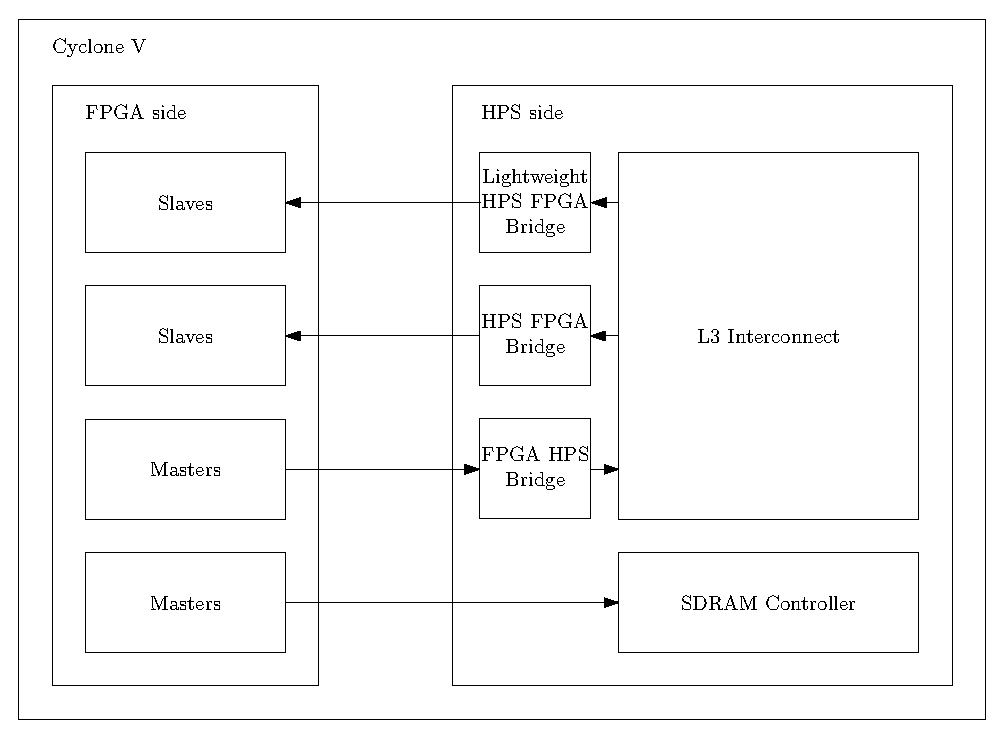
\includegraphics[scale=0.6]{Chapter1-Hardware/res/cycv_interconnect}
    \caption{Interconnect bridges}
    \label{fig:cyc5/interconnect}
\end{figure}

In Figure \ref{fig:cyc5/address_space} the address mappings from different viewpoints are shown. For 
the two buses going from the HPS to the FPGA, it is the MPU column (Memory Protection Unit, the unit 
that protects memory accesses on ARM architectures) that will be of interest. We see that the address 
space is much larger for the hps-fpga bridge than for its lightweight equivalent. These addresses 
are those to which the slaves on the fpga side will be associated and therefore those to which one
will have to send the transactions from the ARM processor in order to communicate with these slaves. 
The protocol will of course be studied in this document but this will be done when the transactions 
between the two parts will be discussed.

\begin{figure}[H]
    \centering
    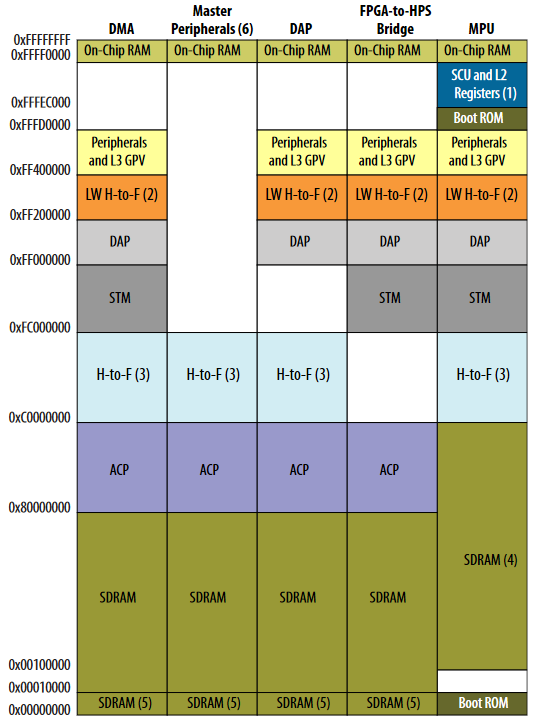
\includegraphics[scale=0.6]{Chapter1-Hardware/res/hps_address_space.PNG}
    \caption{Address maps for system interconnect masters}
    \label{fig:cyc5/address_space}
\end{figure}

\section{On-board and on-chip memories comparison}

As seen in the previous sections, several types of memories are available. Directly on the board 
there is the SD card storage and DDR3 RAM memory. On the Cyclone V there are also two types of memory 
which are MLAB units and M10K blocks. Each memory has its own specificities. Since both the beta 
machine and the ARM system require memory, it is interesting to consider the use of these different 
memories, compare them and finally make a choice.

Let's start with the simplest, the ARM processor. In fact, on this side no choice is left to the 
user. The DDR3 memory will serve as the main memory and the SD card as the secondary memory for 
non-volatile storage. 

Concerning the Beta machine, things are getting tougher.  Which memory to choose to store 
instructions and data, as main memory? Given the nature of SD card memory, it can immediately be 
taken out of the possible choices. What about the other memories?

\subsection{DDR3 memory}

The DDR3 memory offers 1GB 
shareable between the ARM processor and the beta machine, which is really huge. However, an almost 
direct access to this memory is only possible if the access is done in a non-caching and 
non-coherent way with respect to the ARM processor caches. Another possibility is to use the ACP 
ID mapper which will ensure a cached and coherent access (using the L2 cache). The two access paths 
are identified in Figure \ref{fig:de10/ddr3}. The problem with these two accesses is that they are 
not instantaneous, the writes and reads do not take the same number of cycles and the number of 
cycles is not unitary. To use these memories, it is therefore necessary to either slow down the 
whole beta machine or to have a cache memory on the beta machine with faster memory next to it. In 
addition to this, in the first case (direct access) it will be necessary to configure the operating 
system on the ARM processor to ensure that it will never accesses the part of memory reserved for the
beta machine and in the second case (with the ACP) it will be necessary to configure the ACP 
correctly so that its operation is as expected. In both cases this means modifying the kernel of the 
operating system, which is not necessarily simple. For these two reasons: the delays and the 
necessary modifications at the kernel level, this memory has not been chosen. However, it could be 
a very interesting modification of the machine to provide more memory to the system.

\begin{figure}[H]
    \centering
    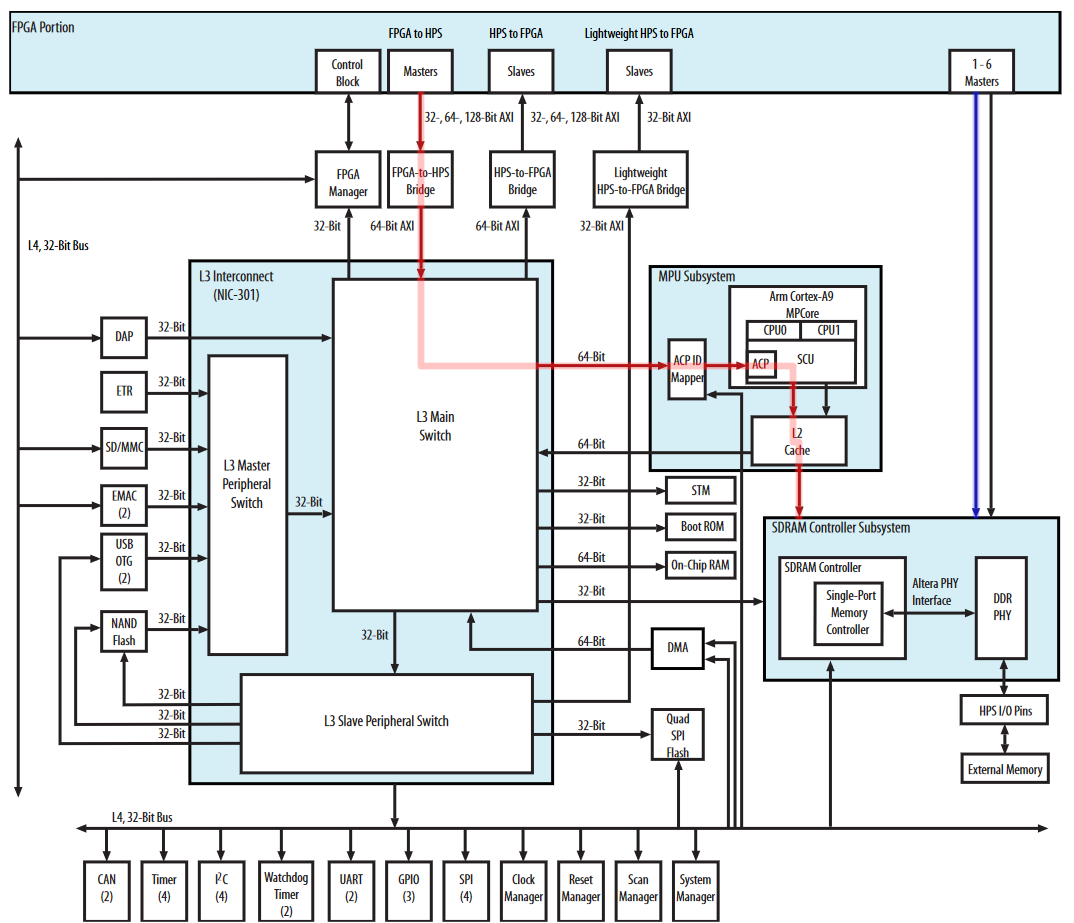
\includegraphics[scale=0.4]{Chapter1-Hardware/res/de10_DDR3.PNG}
    \caption{DDR3 accesses from the FPGA. Red path uses the ACP and blue path is a direct access
    to the memory controler.}
    \label{fig:de10/ddr3}
\end{figure}

\subsection{M10K and MLAB memories}

What about the M10K and MLAB memories? These two memories are directly present on the FPGA, which
 means that they can be read and written in one clock cycle. Moreover, they will not be used by the 
 ARM processor, which avoids having to take care of the coherence of the caches. How to choose 
 between these two memories? The first difference is the amount of memory available. Indeed, the 
 M10K are present in the number of 553 on the Cyclone V SE A6 used in this work. As a M10K memory 
 contains 10Kb, the whole of these blocks represents a little more than 5Mb which is already very 
 important for a machine like the beta machine. The MLABs on their side are present in the number of 
 994 with 640 bits per block as seen previously. This makes a total of a little more than 600kb. 
 However, there are three reasons why the choice will be made for the M10K rather than the MLABs. 
 The first reason is that MLABs consume programmable logic, the more MLAB memory is used the less 
 custom logic can be added to the FPGA, up to a loss of 25\% if all memory is used. The second is 
 that the datasheet advises to use these memories in cases where shallow and large memories are 
 needed. This is because it will be complicated to create large memories locally with MLABs. Last 
 but not least, MLABs do not provide dual-port access, which is a huge handicap because it is 
 necessary to duplicate the memories if the user wants this kind of access. As the choice of M10Ks 
 seems to be the most suitable for this work, it is decided to use only this source of memory and 
 not a hybrid system which keeps things simple. Another difference between MLABs and M10Ks is that 
 MLABs have no problem running at frequencies up to 420MHz while M10Ks do not go beyond 315MHz. 
 However, the beta machine will not exceed a clock frequency of 50MHz which puts this feature out 
 of consideration.